\begin{itemize}
	\item Ensemble de mot sur un alphabet donné
	\item Base de toutes les activités humaines
	\\ Intérêt dans notre cas
	\item Reconnaissance d'un mot d'un langage
	\item Génération d'un mot
	\item Classification des langages
\end{itemize}

\center
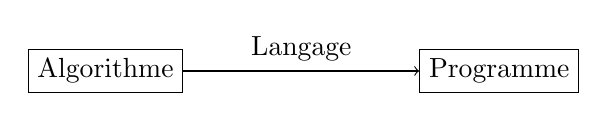
\begin{tikzpicture}[auto]
    \node[draw] at (0, 0) (a) {Algorithme};
    \node[draw] at (5, 0) (p) {Programme};
    \path[->] (a) edge node {Langage} (p);
\end{tikzpicture}

\flushleft
Exemple sur le 10e problème d'Hilbert :
\paragraph{}
On donne une équation de Diophante à un nombre quelconque d'inconnues et à coefficients entiers rationnels : On demande de trouver une méthode par laquelle, au moyen d'un nombre fini d'opérations, on pourra distinguer si l'équation peut être résolue en nombre entiers rationnels.
\paragraph{}
C'est à dire trouver un algorithme pour dire si oui ou non ce genre de polynôme peut être résolue en nombre entiers rationnels :\\
\paragraph{}
\begin{math}
P(a_1,a_2,...,a_n,x_1,x_2,...,x_m) = 0
\end{math}
où P est un polynôme a plusieurs variables et à coefficients entiers.
Les $a_i$ sont les les inconnus, les $x_j$ les paramètres.

\paragraph{}
Pour résoudre ce problème, Church, Turing et d'autres ont du définir formellement ce qu'est un algorithme.
On parlait à l'époque de fonction primitives récursives, $\lambda$-calcul mais on parlera dans ce cours d'algorithmes.

\paragraph{}
Définition précise d'un langage de programmation
-> Outils pour vérifier la syntaxe d'un programme écrit dans un langage de programmation.

\begin{itemize}
	\item Compilateur
	\item Analyse syntaxique / lexicale
\end{itemize}
\paragraph{}
\begin{tabular}{|l|l|l|}
	\hline
	Classe de langage & Reconnaissance de mot & Génération de mot \\
	\hline
	Langage régulier (rationnel) & Automate fini & Grammaire régulière \\
	\hline
	Langage algébrique & Automate à Pile & Grammaire algébrique \\
	\hline
	Langage récursif & Machine de Turing & Grammaire générale \\
	\hline
\end{tabular}

\center
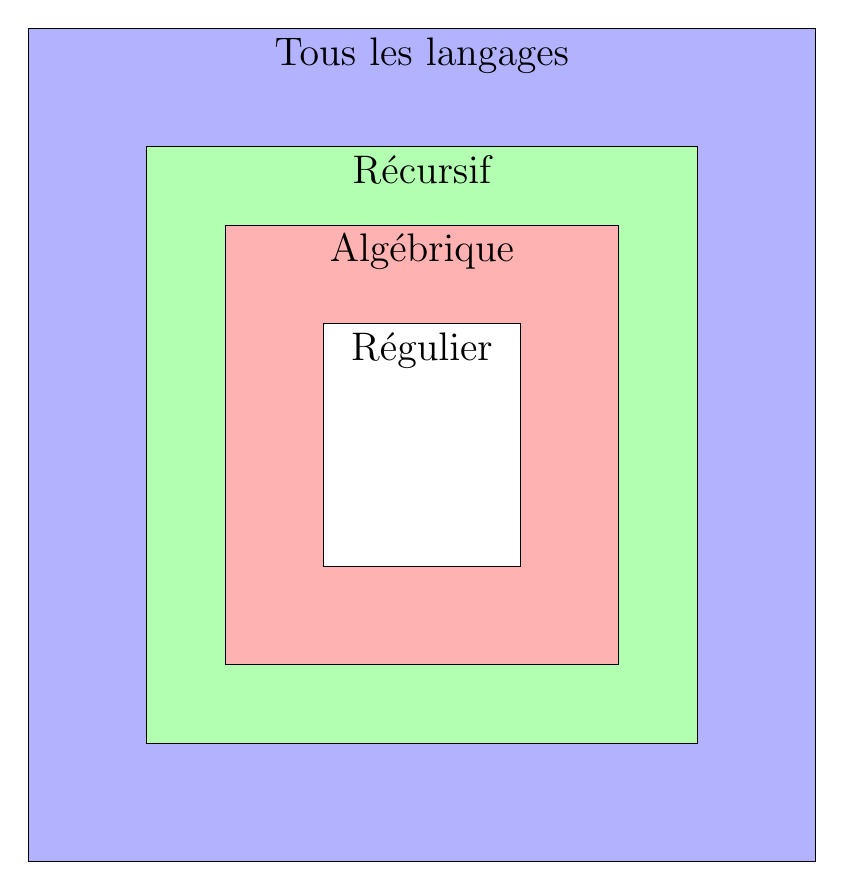
\begin{tikzpicture}
\node[draw,fill=blue!30,text depth=10cm,minimum width=10cm,font=\Large](main){Tous les langages};
\node[draw,fill=green!30,text depth=7cm,minimum width=7cm,font=\Large] at (main.center){Récursif};
\node[draw,fill=red!30,text depth=5cm,minimum width=5cm,font=\Large] at (main.center){Algébrique};
\node[draw,fill=white!30,text depth=2.5cm,minimum width=2.5cm,font=\Large] at (main.center){Régulier};
\end{tikzpicture}
\flushleft